\section*{Problema 2}
\textbf{Let}
\begin{equation}
      f(x) = \frac{xcos(x)-sin(x)}{x-sin(x)}
      \label{eq:problem2fx}
\end{equation}
\begin{enumerate}
      \item \textbf{Find} $\underset{x\rightarrow 0}{lim} f(x)$

            Como queremos entrar el límite cuando x tiende a 0 de la ecuación \ref{eq:problem2fx}. Tenemos que comprobar si el límite por la izquierda y por la derecha es igual. Esto es:

\begin{equation*}
    \underset{x\rightarrow 0^-}{lim} f(x) = L_i
    \qquad
    \underset{x\rightarrow 0^+}{lim} f(x) = L_s
\end{equation*}
El límite existira si y solo sí $L_i=L_s=L$ y es igual a L. Como el límite que queremos comprobar se encuentra en 0, realizaremos esta busqueda a partir del intervalo $[-1,1]$. En cada iteración este intervalo se ira reduciendo una cuarta parte, esto es que en la siguiente iteración el intervalo será $[-0.5,0.5]$. Así hasta obtener una diferencia de $L_i$ y $L_s$ menor a $10^{-6}$ o al haber realizado 16 iteraciones.

El programa arrojo los resultados mostrados en la tabla \ref{table:limiteizquierda} y \ref{table:limitederecha}.
\begin{figure}[H]
    \centering
    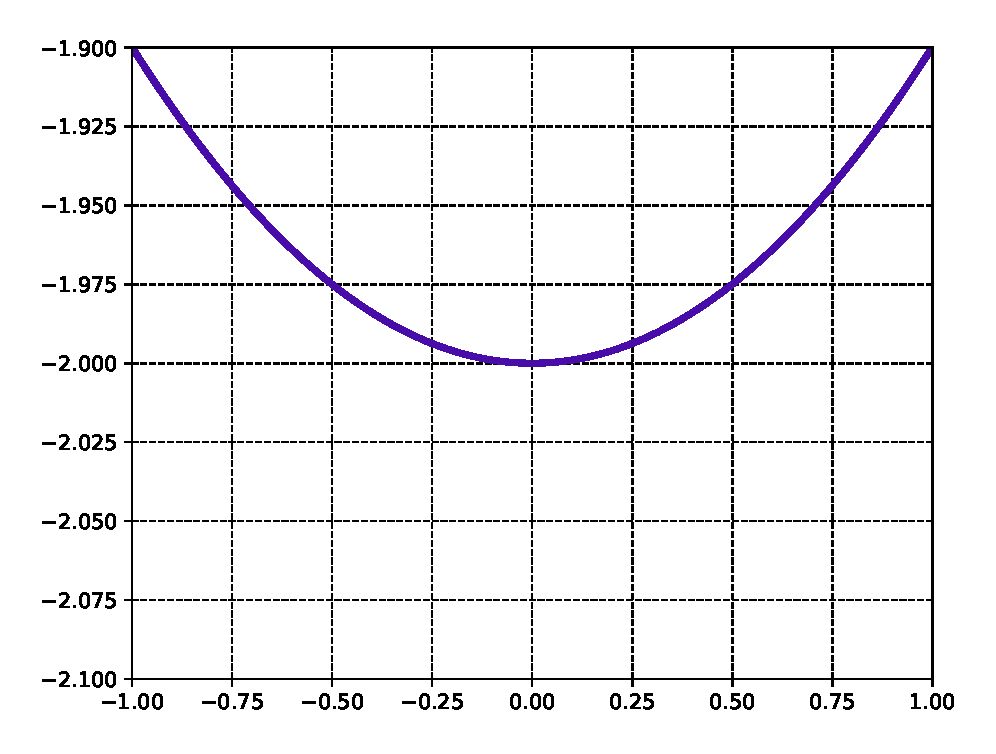
\includegraphics[width=10cm]{Graphics/limit.eps}
    \caption{}
    \label{fig:fx2}
\end{figure}
\begin{minipage}{0.45\linewidth}
    \begin{table}[H]
        \centering
        \begin{tabular}{ll}
            \hline
            \multicolumn{1}{c}{\textbf{x}} & \multicolumn{1}{c}{$\mathbf{L_i}$} \\ \hline
            -1.000000                      & -1.899770                          \\
            -0.500000                      & -1.974985                          \\
            -0.250000                      & -1.993749                          \\
            -0.125000                      & -1.998437                          \\
            -0.062500                      & -1.999609                          \\
            -0.031250                      & -1.999902                          \\
            -0.015625                      & -1.999976                          \\
            -0.007812                      & -1.999994                          \\
            -0.003906                      & -1.999998                          \\
            -0.001953                      & -2.000000                          \\
            -0.000977                      & -2.000000                          \\
            -0.000488                      & -2.000000                          \\ \hline
        \end{tabular}
        \caption{Valores obtenidos para el límite por la izquierda para una x dada.}
        \label{table:limiteizquierda}
    \end{table}
\end{minipage}
\hspace{0.5cm}
\begin{minipage}{0.45\linewidth}
    \begin{table}[H]
        \centering
        \begin{tabular}{ll}
            \hline
            \multicolumn{1}{c}{\textbf{x}} & \multicolumn{1}{c}{$\mathbf{L_s}$} \\ \hline
            1.000000                       & -1.899770                          \\
            0.500000                       & -1.974985                          \\
            0.250000                       & -1.993749                          \\
            0.125000                       & -1.998437                          \\
            0.062500                       & -1.999609                          \\
            0.031250                       & -1.999902                          \\
            0.015625                       & -1.999976                          \\
            0.007812                       & -1.999994                          \\
            0.003906                       & -1.999998                          \\
            0.001953                       & -2.000000                          \\
            0.000977                       & -2.000000                          \\
            0.000488                       & -2.000000                          \\ \hline
        \end{tabular}
        \caption{Valores obtenidos para el límite por la derecha para una x dada.}
        \label{table:limitederecha}
    \end{table}
\end{minipage}

Observando los resultados de las tablas \ref{table:limiteizquierda} y \ref{table:limitederecha} podemos decir que el límite buscado sí existe y es igual a -2. El programa llega a la misma conclusión. En la figura \ref{fig:fx2} se puede verificar la misma conclusión.
\pagebreak
      \item \textbf{Use four-digit rounding arithmetic to evaluate} $f(0.1)$

            La forma en la cual se realizo el calculo es la siguiente. Sea round(x) una función la cual redondea a cuatro decimales, entonces la ecuación \ref{eq:problem2fx} es escrita como:
\begin{equation}
    f_b(x) = round\left(\frac{round(x'sin(x)'cos(x)'))}{round(x'-sin(x)')}\right)
    \label{eq:problema2b}
\end{equation}

donde $sin(x)', cos(x)'$ y $x'$ son los valores de $sin(x),cos(x)$ y $x'$ redondeados a cuatro decimales respectivamente. Evaluando la ecuación \ref{eq:problema2b} en $x=0.1$ se obtiene que $f'(x)$ es igual a $49.5000$.


      \item \textbf{Replace each trigonometric function with its third Maclaurin polynomial and repeat part (b).}

            Escribiendo las ecuaciones de seno y coseno como sereis de potenicas, se obtiene lo siguiente:
\begin{equation*}
    sin(x) = \sum_{i=0}^n \frac{(-1)^i}{(2i+1)!} x^{2i+1} \qquad
    cos(x) = \sum_{i=0}^n \frac{(-1)^i}{(2i)!} x^{2i} \qquad
\end{equation*}

Transformando estas ecuaciones a una ecuación recursiva se obtiene que

\begin{minipage}{0.45\linewidth}
    para $sin(x)$ es
    \begin{align*}
        P_0 & = a_n                  \\
        P_1 & = a_{n-1} + x^2P_0     \\
        P_2 & = a_{n-2} + x^2P_1     \\
            & \qquad\vdots           \\
        P_i & = a_{n-i} + x^2P_{i-1} \\
            & \qquad\vdots           \\
        P_n & = xP_n
    \end{align*}
\end{minipage}
\begin{minipage}{0.45\linewidth}
    En el caso de $cos(x)$ es:
    \begin{align*}
        P_0 & = a_n                  \\
        P_1 & = a_{n-1} + x^2P_0     \\
        P_2 & = a_{n-2} + x^2P_1     \\
            & \qquad\vdots           \\
        P_i & = a_{n-i} + x^2P_{i-1} \\
            & \qquad\vdots           \\
        P_n & = a_{n-1}+x^2P_{n-1}
    \end{align*}
\end{minipage}

Por lo tanto, la ecuación que se calculara es la siguiente:
\begin{equation}
    f_c(x) = \frac{x \left(\sum\limits_{i=0}^{n=2} \frac{(-1)^i}{(2i+1)!}\right) \left(x^{2i+1}\sum\limits_{i=0}^{n=2} \frac{(-1)^i}{(2i)!} x^{2i}\right)}{x-\sum\limits_{i=0}^{n=2} \frac{(-1)^i}{(2i+1)!} x^{2i+1}}
    \label{eq:problema_fc}
\end{equation}

Evaluando la función en $x=0.1$, se obtiene como resultado que $f(x=0.1)=49.5000$.
      \item \textbf{The actual value is f (0.1) = -1.99899998. Find the relative error for the values obtained in parts (b) and (c).}

            Calculando la diferecia relativa entre los datos obtenidos se obtienen los resultados que se muestran en la tabla \ref{table:results2d}.

\begin{table}[H]
      \centering
      \begin{tabular}{lcc}
            \hline
            \textbf{Función}                                   & \textbf{f(x)} & \textbf{\begin{tabular}[c]{@{}l@{}}Diferencia\\ Relativa\end{tabular}} \\ \hline
            Análitica (Ecuación \ref{eq:problem2fx})           & -1.998999     & -                                  \\
            Redondeo (Ecaución \ref{eq:problema2b})            & -1.500000     & 24.9625                            \\
            Serie de potencias (Ecuación \ref{eq:problema_fc}) & -1.500000     & 24.9625                            \\ \hline
      \end{tabular}
      \caption{Valores obtenidos en los ejercicos 2b y 2c comparandolos con el resultado análitico de la ecuación \ref{eq:problem2fx} en x=0.1.}
      \label{table:results2d}
\end{table}

\end{enumerate}

Con los resultados mostrados en las tablas \ref{table:resultados1} y \ref{table:results2d}  se puede aclarar que el redondear a cuatro decimales la funciones seno y coseno es equivalente a usar hasta el tercer término de la expansión por serie de Maclaurin. El programa se encuentra en la carpeta \textcolor{citecolor}{Problema\_2}. Para compilar el programa se debe ingresar la siguiente linea:
\begin{lstlisting}[language=bash]
      gcc -Wall -Wextra -Werror -pedantic -ansi -o main.out main.c -lm -std=c11
\end{lstlisting}

El output esperado del programa es el siguiente:

\begin{lstlisting}[language=bash]
      ----------------------------------
      x		Li		x		Ls
      -1.000000	-1.899770	1.000000	-1.899770
      -0.500000	-1.974985	0.500000	-1.974985
      -0.250000	-1.993749	0.250000	-1.993749
      -0.125000	-1.998437	0.125000	-1.998437
      -0.062500	-1.999609	0.062500	-1.999609
      -0.031250	-1.999902	0.031250	-1.999902
      -0.015625	-1.999976	0.015625	-1.999976
      -0.007812	-1.999994	0.007812	-1.999994
      -0.003906	-1.999998	0.003906	-1.999998
      -0.001953	-2.000000	0.001953	-2.000000
      -0.000977	-2.000000	0.000977	-2.000000
      -0.000488	-2.000000	0.000488	-2.000000
      
      El limite cuando f(x) tiende a cero es -2.000000
      
      ----------------------------------
      El valor de f(x)
            Con series es: -1.5000
            Con redondeo a 4 decimales es: -1.5000
      
      ----------------------------------
      La diferencia relativa de f(x)
            Con redondeo a 4 decimales es: 24.9625
            Con series es: 24.9625
\end{lstlisting}
